\chapter{Конструкторский раздел}
\label{cha:design}
В данном разделе будут рассмотрены схемы алгоритма полного перебора, бинарного поиска и сегментации.

\section{Схемы базовых алгоритмов}
\label{sec:schemes}
На рисунке \ref{fig:fullsearch} представлена схема поиска полным перебором.
\begin{figure}[H]
	\centering
	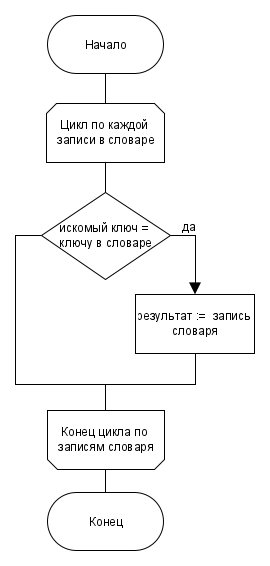
\includegraphics[width=0.5\linewidth]{src/fullsearch}
	\caption{Полный перебор}
	\label{fig:fullsearch}
\end{figure}

На рисунке \ref{fig:binsearch} представлена схема поиска двоичным перебором.
\begin{figure}[H]
	\centering
	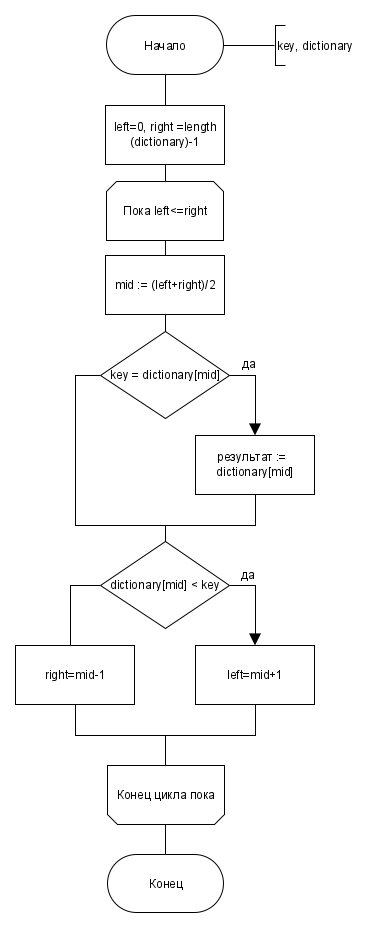
\includegraphics[height=0.7\textheight]{src/binsearch}
	\caption{Двоичный поиск}
	\label{fig:binsearch}
\end{figure}


\section{Частотный анализ}
\label{sec:freq}
В качестве 3-его алгоритма была реализована сегментация вместе с частотным анализом. Частотный анализ проводится по первому символу ключа, как и сегментация. В результате получается множество сегментов, упорядоченных по убыванию частоты первого символа. Наиболее короткие сегменты объединяются, пока их суммарная длина не будет выше константы. На рисунке \ref{fig:segmentation} представлена схема алгоритма сегментирования словаря.
\begin{figure}[H]
	\centering
	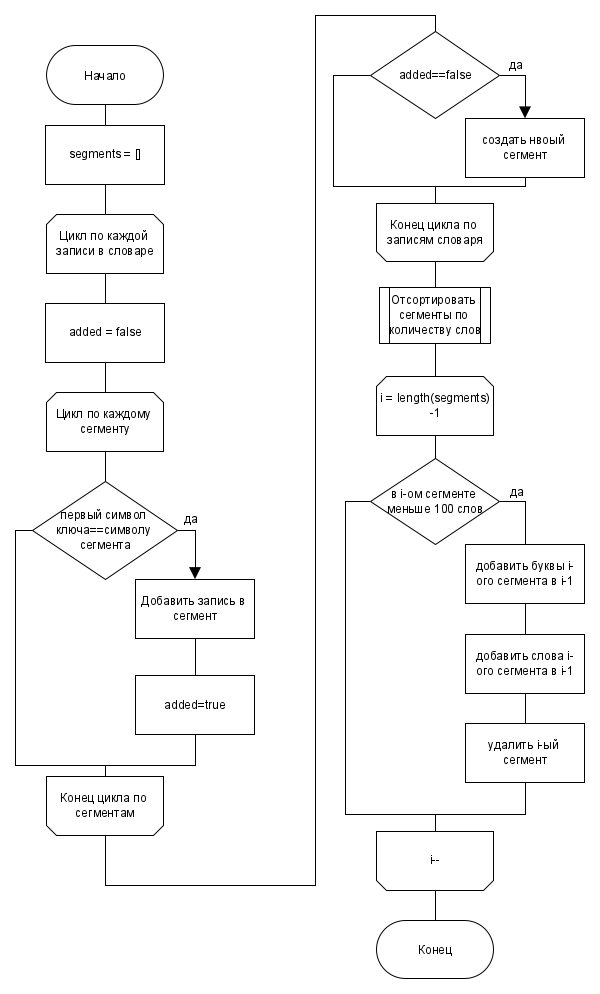
\includegraphics[height=0.8\textheight]{src/segmentation}
	\caption{Алгоритм сегментации}
	\label{fig:segmentation}
\end{figure}
После чего полученные сегменты используются для поиска, на рисунке \ref{fig:segsearch} представлен алгоритм поиска в сегменте.
\begin{figure}
	\centering
	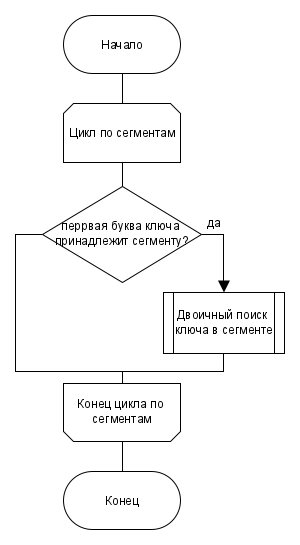
\includegraphics[width=0.5\linewidth]{src/segsearch}
	\caption{Поиск с использованием сегментов}
	\label{fig:segsearch}
\end{figure}


\section{Вывод}
\label{sec:design_conclusion}
В данном разделе были рассмотрены схемы алгоритма полного перебора и двоичного поиска, а также сегментирования.